% =====================================================================
%  Internship Report — Mobile Application Developer Intern
%  at Power Gym Budibazar Pokhara
%
%  MASTER FILE.  Compile from inside this directory:
%      latexmk -xelatex main.tex
%  or run  .\build.ps1
%
%  Format specification:  config/preamble.tex   (input below)
%  Names and numbers:     config/metadata.tex   (input below)
%  Helpers:               config/macros.tex     (input below)
%  Format rules:          docs/guidelines/guidelines.md
%  Plan and open decisions: docs/imp/plan.md
%  Content sources:       docs/project_detail/
% =====================================================================
\documentclass[12pt,a4paper,oneside]{report}

% =====================================================================
%  PREAMBLE — the whole format specification in one place.
%  main.tex inputs this file right after \documentclass.
%
%  Every line here is verified against docs/guidelines/guidelines.md:
%    Times New Roman 12pt, A4, margins T1 B1 R1 L1.25 (main matter),
%    justified 1.5 spacing, chapter 16 / section 14 / subsection 12 bold,
%    caption below figures and above tables, bold 12pt centred,
%    page number bottom centre, APA citations.
%
%  Do not re-implement any of this elsewhere; record any deliberate
%  change in docs/imp/plan.md.
% =====================================================================

% ---------------------------------------------------------------------
% 1. Fonts — Times New Roman (real system font, XeLaTeX)
%    unicode-math gives Times-compatible maths. Without it the maths used
%    in the architecture diagram pulls in Computer Modern (CMSY/CMEX) and the
%    guideline's "Times New Roman only" requirement is broken.
% ---------------------------------------------------------------------
\usepackage{fontspec}
\setmainfont{Times New Roman}
\usepackage{unicode-math}
\setmathfont{TeX Gyre Termes Math}

% ---------------------------------------------------------------------
% 2. Page geometry — A4, top 1in, bottom 1in, right 1in, left 1.25in
%    Open decision D1: guideline states "1" without a unit; inches assumed.
%    The front matter switches to left=1.5in via \newgeometry in main.tex,
%    because that is what the approved Word draft uses (see main.tex).
% ---------------------------------------------------------------------
\usepackage[
  a4paper,
  left=1.25in,
  right=1in,
  top=1in,
  bottom=1in,
  footskip=0.35in
]{geometry}

% ---------------------------------------------------------------------
% 3. Paragraphs — justified, 1.5 line spacing, 0pt indent, 6pt skip
%    Open decision D2: 1.43 reproduces Word's "1.5 lines" for TNR 12pt.
%    \parskip is 0 during the front matter (each gap is an explicit
%    \vspace matching the Word draft) and 6pt from Chapter 1 on.
% ---------------------------------------------------------------------
\usepackage{setspace}
\usepackage{microtype}
\setstretch{1.43}
\setlength{\parindent}{0pt}
\setlength{\parskip}{6pt}
\setlength{\emergencystretch}{3em}   % stop overfull lines with justified text

% ---------------------------------------------------------------------
% 4. Headings — chapter 16pt, section 14pt, sub-section 12pt, all bold
% ---------------------------------------------------------------------
\usepackage{titlesec}
\usepackage{titletoc}

\renewcommand{\chaptername}{CHAPTER}
\renewcommand{\contentsname}{TABLE OF CONTENTS}
\renewcommand{\listfigurename}{LIST OF FIGURES}
\renewcommand{\listtablename}{LIST OF TABLES}

\titleformat{\chapter}[display]
  {\centering\bfseries\fontsize{16}{19}\selectfont}
  {\chaptername\ \thechapter}
  {4pt}
  {}
\titleformat{name=\chapter,numberless}
  {\centering\bfseries\fontsize{16}{19}\selectfont}
  {}
  {0pt}
  {}
\titleformat{\section}
  {\normalfont\bfseries\fontsize{14}{17}\selectfont}
  {\thesection\quad}
  {0pt}
  {}
\titleformat{\subsection}
  {\normalfont\bfseries\fontsize{12}{14}\selectfont}
  {\thesubsection\quad}
  {0pt}
  {}
\titlespacing*{\chapter}{0pt}{0pt}{18pt}
\titlespacing*{name=\chapter,numberless}{0pt}{0pt}{18pt}
\titlespacing*{\section}{0pt}{12pt}{4pt}
\titlespacing*{\subsection}{0pt}{8pt}{3pt}

% Table of Contents layout (titletoc)
\titlecontents{chapter}[0pt]
  {\vspace{0.8em}\bfseries}
  {\chaptername\ \thecontentslabel:\quad}
  {}
  {\titlerule*[0.75pc]{.}\contentspage}

\titlecontents{section}[2.5em]
  {\normalfont}
  {\thecontentslabel\quad}
  {}
  {\titlerule*[0.75pc]{.}\contentspage}

\titlecontents{subsection}[5em]
  {\normalfont}
  {\thecontentslabel\quad}
  {}
  {\titlerule*[0.75pc]{.}\contentspage}

\titlecontents{figure}[2.5em]
  {\normalfont}
  {\contentslabel{2.5em}}
  {}
  {\titlerule*[0.75pc]{.}\contentspage}

\titlecontents{table}[2.5em]
  {\normalfont}
  {\contentslabel{2.5em}}
  {}
  {\titlerule*[0.75pc]{.}\contentspage}

% ---------------------------------------------------------------------
% 5. Figures and tables — caption below figures, above tables,
%    both centred and bold 12pt
% ---------------------------------------------------------------------
\usepackage{graphicx}
\usepackage{float}
\usepackage{caption}
\DeclareCaptionFont{repcap}{\bfseries\fontsize{12}{14}\selectfont}
\captionsetup{
  font=repcap,
  justification=centering,
  singlelinecheck=false,
  labelsep=period
}
\captionsetup[figure]{position=bottom}
\captionsetup[table]{position=top}

% ---------------------------------------------------------------------
% 6. Tables
% ---------------------------------------------------------------------
\usepackage{array}
\usepackage{booktabs}
\usepackage{tabularx}
\usepackage{longtable}

% ---------------------------------------------------------------------
% 7. Lists
% ---------------------------------------------------------------------
\usepackage{enumitem}
\setlist[itemize]{leftmargin=0.5in,itemsep=2pt,topsep=4pt}
\setlist[enumerate]{leftmargin=0.5in,itemsep=2pt,topsep=4pt}

% ---------------------------------------------------------------------
% 8. Source code listings for the appendices
% ---------------------------------------------------------------------
\usepackage{xcolor}
\usepackage{tikz}            % certificate frame drawn on the mentor page only
\usetikzlibrary{calc}
\usepackage{eso-pic}         % background frame on the mentor certificate page
\usepackage{letterspace}     % \textls letterspacing for the certificate title
\usepackage{listings}
\lstset{
  basicstyle=\ttfamily\small,
  breaklines=true,
  breakatwhitespace=true,
  frame=single,
  captionpos=b,
  numbers=left,
  numberstyle=\tiny\color{gray},
  showstringspaces=false
}

% ---------------------------------------------------------------------
% 8b. Mentor certificate — colours and official stamp placeholder
%     Design from suggestions.md, fixed: \OfficialStampName is "Power Gym"
%     (two words, matching data/information/company_information.md and
%     \CompanyName), and the page uses serif \bfseries only so the build
%     keeps embedding Times New Roman exclusively (no \sffamily).
% ---------------------------------------------------------------------
\providecolor{certNavy}{RGB}{15,36,64}
\providecolor{certGold}{RGB}{176,138,58}
\providecolor{certInk}{RGB}{32,38,48}
\providecolor{certSlate}{RGB}{84,94,105}

% Exact wording used in the official stamp section.
\providecommand*{\OfficialStampName}{Power Gym}

% Official stamp placeholder (empty dashed box — left blank for stamping)
\providecommand*{\OfficialStampPlaceholder}{%
  \begin{tikzpicture}[baseline=-1.125cm]
    \node[
      draw=certSlate!80,
      line width=0.8pt,
      dash pattern=on 2.4pt off 2.0pt,
      rounded corners=4pt,
      minimum width=3.35cm,
      minimum height=2.25cm,
      inner sep=0pt
    ] (stampbox) {};
    \draw[
      certSlate!35,
      line width=0.4pt,
      rounded corners=2.8pt
    ]
      ($(stampbox.north west)+(0.15cm,-0.15cm)$)
      rectangle
      ($(stampbox.south east)+(-0.15cm,0.15cm)$);
  \end{tikzpicture}%
}

% ---------------------------------------------------------------------
% 9. Page numbers — bottom centre
% ---------------------------------------------------------------------
\usepackage{fancyhdr}
\pagestyle{fancy}
\fancyhf{}
\renewcommand{\headrulewidth}{0pt}
\renewcommand{\footrulewidth}{0pt}
\fancyfoot[C]{\thepage}

% ---------------------------------------------------------------------
% 10. Citations — natbib with a hand-written APA reference list
%     See plan section 6: every \bibitem needs an explicit APA label.
% ---------------------------------------------------------------------
\usepackage{natbib}

% ---------------------------------------------------------------------
% 11. Hyperlinks — loaded last, invisible
% ---------------------------------------------------------------------
\usepackage[hidelinks]{hyperref}

% ---------------------------------------------------------------------
% 12. Image search paths
%     Resolved relative to src/sections (the build's working directory):
%       figures/        -> src/sections/figures  (screenshots etc.)
%       ../data/figures -> the report's prepared images: TU logo
%                         (tu_logo.png), organization hierarchy, screen
%                         image, company logo.
% ---------------------------------------------------------------------
\graphicspath{{figures/}{../data/figures/}}

% =====================================================================
%  Report metadata — the single source of truth for every name, title
%  and number used by the front matter.  main.tex inputs this file.
%
%  Sources (never invent a value):
%    data/information/front_matter.md
%    docs/zz/Internship_Report_Tirshana_Subedi.docx   (approved Word draft)
%
%  NOTE: this file originally came from a template written for a
%  different student's project ("Krishi Vaidya ... Crop Disease
%  Diagnosis", 26 May 2026, 7th Semester, registration 5-2-48-193-2022).
%  Those values were removed — they are not this report's.  Registration
%  number and submission day are still unknown: see
%  docs/project_detail/12_open_questions_and_discrepancies.md.
% =====================================================================

% --- document -------------------------------------------------------
\newcommand{\ReportTitle}{Internship Report on ``Mobile Application Developer Intern'' at Power Gym Budibazar Pokhara}
\newcommand{\ReportAuthor}{Tirshana Subedi}
\newcommand{\SymbolNumber}{79011927}          % confirmed: printed on cover,
                                              % declaration and acknowledgement
                                              % of the approved Word draft
% TODO: registration number unknown — do not reuse the template's
%       5-2-48-193-2022; ask the department.
\newcommand{\SubmissionMonthYear}{October 2026}
\newcommand{\SemesterName}{8th Semester}

% --- institution ----------------------------------------------------
\newcommand{\CampusFullName}{Prithvi Narayan Campus}
\newcommand{\CampusAddress}{Bhimkalipatan-1, Pokhara}
\newcommand{\InstituteName}{Institute of Science and Technology}
\newcommand{\UniversityName}{Tribhuvan University}
\newcommand{\DepartmentFullName}{Department of Computer Science and Information Technology}
\newcommand{\ProgramName}{B.Sc. CSIT}
\newcommand{\ProgramFullName}{Bachelor of Science in Computer Science and Information Technology}

% --- host organisation ----------------------------------------------
\newcommand{\CompanyName}{Power Gym Budibazar Pokhara}
\newcommand{\InternPosition}{Mobile Application Developer Intern}
\newcommand{\GymManagementName}{Neeraj Tiwari}
\newcommand{\CompanyMentorTitle}{Mr.}
\newcommand{\CompanyMentor}{Krishna Subedi}
% Source: data/information/neryva_collaboration.md (author, 9 Oct 2026)
\newcommand{\CompanyMentorRole}{Senior Software Engineer}
\newcommand{\CompanyMentorOrg}{Neryva}
\newcommand{\CompanyMentorOrgUrl}{neryva.com}
\newcommand{\WorkLocation}{Neryva Lab}

% --- signatories -----------------------------------------------------
\newcommand{\SupervisorTitle}{Mr.}
\newcommand{\SupervisorName}{Gyaneshwor Dhungana}
\newcommand{\HeadOfDepartment}{Chudamani Subedi}
\newcommand{\HeadOfDepartmentTitle}{Program Director}

% --- images -----------------------------------------------------------
%  High-resolution TU logo extracted from the approved Word draft
%  (305 x 354 px).  Resolved through the graphics path declared in
%  config/preamble.tex.
\newcommand{\LogoFile}{tu_logo.png}

\newcommand{\PrelimHeading}[1]{%
  \clearpage
  \thispagestyle{plain}
  {\noindent\bfseries\fontsize{16}{18}\selectfont #1\par}
  \vspace{1.5\baselineskip}
}

\newcommand{\PrelimEntry}[1]{}

\newcommand{\ChapterSection}[1]{%
  \section{#1}
}

\newcommand{\ChapterSubsection}[1]{%
  \subsection{#1}
}

\newcommand{\DashedSignatureLine}[1]{%
  \noindent\makebox[#1][l]{%
    \xleaders\hbox{-\kern0.5pt}\hfill\kern0pt%
  }%
}

\newcommand{\SignatureBlock}[5]{%
  \vspace{2\baselineskip}
  \DashedSignatureLine{6cm}\\
  #1\\
  #2\\
  #3\\
  #4\\
  #5
}

\newcommand{\TitleCaseLine}[1]{%
  \begin{center}
    \bfseries\fontsize{14}{16}\selectfont\MakeUppercase{#1}
  \end{center}
}

\newcommand{\CenteredBodyLine}[1]{%
  \begin{center}
    \fontsize{14}{16}\selectfont #1
  \end{center}
}

\newcommand{\UseIndentedPars}{%
  \setlength{\parindent}{1.27cm}%
  \setlength{\parskip}{0pt}%
}

\newcommand{\UseNoIndentPars}{%
  \setlength{\parindent}{0pt}%
  \setlength{\parskip}{0.5\baselineskip}%
}

\newcommand{\CenteredTOC}{%
  \PrelimHeading{Table of Contents}%
  \PrelimEntry{Table of Contents}%
  \tableofcontents
}

\newcommand{\CenteredLOF}{%
  \PrelimHeading{List of Figures}%
  \PrelimEntry{List of Figures}%
  \listoffigures
}

\newcommand{\CenteredLOT}{%
  \PrelimHeading{List of Tables}%
  \PrelimEntry{List of Tables}%
  \listoftables
}


% =====================================================================
%                              DOCUMENT
% =====================================================================
\begin{document}

% ---------------------------------------------------------------------
%  Front matter geometry.
%    The approved Word draft (docs/zz/Internship_Report_Tirshana_Subedi.docx)
%    lays the front pages out with a 1.5in left margin; the guideline's
%    1.25in is restored for Chapter 1 onwards with \restoregeometry below.
%    Front matter also uses \parskip 0pt: every gap is an explicit
%    \vspace copied from the Word draft's paragraph spacing.
% ---------------------------------------------------------------------
\newgeometry{top=1in,bottom=1in,left=1.5in,right=1in,footskip=0.35in}
\setlength{\parskip}{0pt}
% Word does not hyphenate on these pages, and hyphenation changes where
% justified lines break, which shifts every word on the line. Match it.
\hyphenpenalty=10000
\exhyphenpenalty=10000

% ---------------------------------------------------------------------
%  Cover page — no page number (titlepage sets the style to empty)
% ---------------------------------------------------------------------
% =====================================================================
%  Cover and Title Page
%  Text taken from data/documents/front.pdf page 1. Do not rewrite names,
%  titles or the roll number (data/information/front_matter.md).
%
%  No page number is printed: the titlepage environment sets the page style
%  to empty. The vertical spacing below is tuned so the whole cover fits on
%  a single A4 page — verify after any edit:
%     pdftotext -f 2 -l 2 main.pdf - | Select-Object -First 1
%  must return the certificate page, not cover text.
% =====================================================================
\begin{titlepage}
\centering
\setstretch{1.0}          % the cover is a display page, not body text

\vspace*{0.25in}

% University logo. The source file is only 156 x 181 px, so it must stay
% small: about 1.0in wide. Optionally replace it with the higher-resolution
% version embedded in front.pdf (305 x 354 px).

\includegraphics[width=1.0in]{tribhuwan_university_logo.png}

\vspace{0.22in}

{\bfseries\fontsize{14}{16}\selectfont Prithvi Narayan Campus\par}
{\bfseries\fontsize{14}{16}\selectfont Tribhuvan University\par}
{\bfseries\fontsize{14}{16}\selectfont Institute of Science and Technology\par}

\vspace{0.5in}

{\bfseries\fontsize{16}{19}\selectfont An Internship Report\par}
\vspace{0.06in}
{\bfseries\fontsize{16}{19}\selectfont on\par}
\vspace{0.14in}
{\bfseries\fontsize{16}{19}\selectfont ``Mobile Application Developer Intern''\par}
\vspace{0.06in}
{\bfseries\fontsize{16}{19}\selectfont at\par}
\vspace{0.14in}
{\bfseries\fontsize{16}{19}\selectfont Power Gym Budibazar Pokhara\par}

\vspace{0.42in}

{\bfseries\fontsize{12}{14}\selectfont Submitted To:\par}
\vspace{0.04in}
{\fontsize{12}{14}\selectfont
Department of Computer Science and Information Technology\par
B.Sc. CSIT Program, Prithvi Narayan Campus\par
Bhimkalipatan-1, Pokhara\par}

\vspace{0.34in}

{\fontsize{12}{14}\selectfont
In partial fulfillment of the requirements for the degree of\par
Bachelor of Science in Computer Science and Information Technology\par}

\vspace{0.38in}

{\bfseries\fontsize{12}{14}\selectfont Submitted By:\par}
\vspace{0.04in}
{\fontsize{12}{14}\selectfont
Tirshana Subedi\par
Roll No: 79011927\par
% OPEN QUESTION: data/information/front_matter.md marks the roll number
% "[CONFIRM: 79011927 ]". The cover page of front.pdf prints 79011927 while
% its acknowledgement page prints 79011. Use the confirmed value here AND
% in acknowledgement.tex, or nowhere.
B.Sc. CSIT Program\par}

\vspace{0.34in}

{\bfseries\fontsize{12}{14}\selectfont October 2026\par}

\end{titlepage}

% ---------------------------------------------------------------------
%  Roman-numbered front matter, starting at i on the first certificate page
%  NOTE: \frontmatter does not exist in the report class; it is done by hand.
% ---------------------------------------------------------------------
\clearpage
\pagenumbering{roman}

% =====================================================================
%  Mentor's Recommendation from the Company
%
%  *** TEXT MISSING — THIS PAGE CANNOT BE COMPLETED YET ***
%
%  docs/guidelines/guidelines.md requires three certificate pages:
%    (i)  Mentor's Recommendation from the Company   -> this file
%    (ii) Supervisor's Recommendation      -> certificate-supervisor.tex
%    (iii) Examiners' Approval Letter      -> letter-of-approval.tex
%
%  Neither data/documents/front.pdf nor the approved Word draft
%  (docs/zz/Internship_Report_Tirshana_Subedi.docx) contains this page —
%  the Word file starts straight at the Supervisor's Recommendation.
%  The wording must be supplied; the signatory is either the internship
%  mentor Mr. Krishna Subedi (data/information/company_information.md)
%  or the gym management, Neeraj Tiwari (data/information/front_matter.md)
%  — OPEN QUESTION, confirm before filling in.
%
%  The page is laid out like the other certificate pages (header, logo,
%  underlined 14pt title) so it slots in correctly once the text arrives.
%  This page carries roman page number i (it is the first certificate page).
% =====================================================================
\clearpage

{\centering
{\bfseries\fontsize{16}{19.3}\selectfont \CampusFullName\par}
\vspace{3pt}
{\bfseries\fontsize{16}{19.3}\selectfont \UniversityName\par}
\vspace{3pt}
{\bfseries\fontsize{16}{19.3}\selectfont \InstituteName\par}
\vspace{10pt}
\includegraphics[width=1.04in]{\LogoFile}\par
\vspace{12pt}
{\setstretch{1}\bfseries\fontsize{14}{16.1}\selectfont\underline{MENTOR'S RECOMMENDATION}\par}
\vspace{12pt}

}

% TODO: paste the approved wording here once received. It should follow the
% same pattern as the supervisor's recommendation: who the report was
% prepared by, what the intern did, and a recommendation for evaluation.
{\itshape [Placeholder — the company mentor's recommendation has not yet
been supplied. This page is required by the university guideline and must
be replaced with the approved text before submission.]}

\vspace{62.1pt}
\vspace{13.8pt}
\vspace{13.45pt}
\noindent\rule{1.91in}{2.25pt}
\vspace{13pt}

% OPEN QUESTION: confirm the signatory — internship mentor or gym management.
{\bfseries\fontsize{12}{14.5}\selectfont \CompanyMentorTitle\ \CompanyMentor\par}
\vspace{5.3pt}
{\bfseries\fontsize{12}{14.5}\selectfont Internship Mentor\par}
\vspace{5.45pt}
{\bfseries\fontsize{12}{14.5}\selectfont \CompanyName\par}

% =====================================================================
%  Supervisor's Recommendation
%  Text taken from data/documents/front.pdf page 2.
%  This is the first roman-numbered page (i).
%
%  Signature block: leave blank for hand signing. Rule lines are drawn
%  with \rule so the student can sign above them.
% =====================================================================
\clearpage
\begin{center}

\includegraphics[width=1.1in]{tribhuwan_university_logo.png}\\[0.3in]
{\bfseries Prithvi Narayan Campus}\\
{\bfseries Tribhuvan University}\\
{\bfseries Institute of Science and Technology}
\end{center}

\vspace{0.4in}

\begin{center}
{\bfseries\fontsize{14}{17}\selectfont SUPERVISOR'S RECOMMENDATION}
\end{center}

\vspace{0.2in}

I hereby recommend this internship report prepared under my supervision by Tirshana Subedi, a
B.Sc. CSIT student at Prithvi Narayan Campus, in partial fulfillment of the requirements for the
B.Sc. CSIT degree. During her internship, I observed her consistent dedication and steady progress
in all assigned tasks. Her work meets the academic and professional standards set by the Institute of
Science and Technology at Tribhuvan University.

I confirm that she has satisfactorily completed her internship under my guidance and recommend this
report for final evaluation.

\vspace{1.2in}

\begin{flushright}
\begin{tabular}{@{}c@{}}
\rule{2.6in}{0.4pt}\\
\textbf{Mr. Gyaneshwor Dhungana}\\
Internship Supervisor\\
B.Sc. CSIT Program
\end{tabular}
\end{flushright}
% =====================================================================
%  Letter of Approval
%  Text taken from data/documents/front.pdf page 3.
%  Four signature blocks, arranged two by two.
%
%  OPEN QUESTION: the internal and external examiner names are unknown.
%  Do not copy them from docs/samples/sample 1.docx or sample 2.pdf —
%  those are other students' reports.
% =====================================================================
\clearpage
\begin{center}

\includegraphics[width=1.1in]{tribhuwan_university_logo.png}\\[0.3in]
{\bfseries Prithvi Narayan Campus}\\
{\bfseries Tribhuvan University}\\
{\bfseries Institute of Science and Technology}
\end{center}

\vspace{0.4in}

\begin{center}
{\bfseries\fontsize{14}{17}\selectfont LETTER OF APPROVAL}
\end{center}

\vspace{0.2in}

This is to certify that the internship report submitted by Ms. Tirshana Subedi, a student of Bachelor
of Science in Computer Science and Information Technology program at Prithvi Narayan Campus, has been
evaluated in accordance with the guidelines of the Institute of Science and Technology, Tribhuvan
University, for partial fulfillment of the B.Sc. CSIT degree.

The report meets the required academic and professional standards and is approved for final
evaluation.

\vspace{1.0in}

\noindent
\begin{minipage}[t]{0.47\textwidth}
\centering
\rule{2.3in}{0.4pt}\\
\textbf{Mr. Chudamani Subedi}\\
Program Director\\
Prithvi Narayan Campus
\end{minipage}
\hfill
\begin{minipage}[t]{0.47\textwidth}
\centering
\rule{2.3in}{0.4pt}\\
\textbf{Mr. Gyaneshwor Dhungana}\\
Internship Supervisor\\
Prithvi Narayan Campus
\end{minipage}

\vspace{1.0in}

\noindent
\begin{minipage}[t]{0.47\textwidth}
\centering
\rule{2.3in}{0.4pt}\\
% OPEN QUESTION: confirm the internal examiner's name.
\textit{Internal Examiner}\\
Prithvi Narayan Campus
\end{minipage}
\hfill
\begin{minipage}[t]{0.47\textwidth}
\centering
\rule{2.3in}{0.4pt}\\
% OPEN QUESTION: confirm the external examiner's name.
\textit{External Examiner}\\
Prithvi Narayan Campus
\end{minipage}

% TODO: the external examiner's affiliation is usually printed under the
% name. Confirm the wording with the department.
% =====================================================================
%  Student's Declaration
%  Text taken from data/documents/front.pdf page 4.
%  Mentions the APA reference standard, as the guidelines require.
% =====================================================================
\clearpage
\begin{center}

\includegraphics[width=1.1in]{tribhuwan_university_logo.png}\\[0.3in]
{\bfseries Prithvi Narayan Campus}\\
{\bfseries Tribhuvan University}\\
{\bfseries Institute of Science and Technology}
\end{center}

\vspace{0.4in}

\begin{center}
{\bfseries\fontsize{14}{17}\selectfont STUDENT'S DECLARATION}
\end{center}

\vspace{0.2in}

I hereby declare that the internship report entitled ``Mobile Application Developer Intern'',
submitted to the Institute of Science and Technology, Tribhuvan University, in partial fulfillment of
the requirements for the degree of Bachelor of Science in Computer Science and Information Technology
(B.Sc. CSIT), is the result of work undertaken by me during my internship at Power Gym Budibazar
Pokhara.

This report has not been submitted to any other institution for the award of any degree or diploma.
I have properly acknowledged and cited all the sources of information used in this report in
accordance with the APA reference standard.

I further declare that the tasks presented in this report are genuine and were completed during the
internship period at Power Gym Budibazar Pokhara.

\vspace{1.2in}

\noindent
\begin{tabular}{@{}l@{}l@{}}
Submitted By: & Tirshana Subedi\\
              & Roll No: 79011927\\
              & B.Sc. CSIT Program\\
              & Prithvi Narayan Campus, Pokhara
\end{tabular}
% =====================================================================
%  Acknowledgement
%  Text taken from data/documents/front.pdf page 5.
%  Signatory block at the bottom right, blank for hand signing.
% =====================================================================
\clearpage
\addcontentsline{toc}{chapter}{Acknowledgement}

I would like to express my sincere gratitude to everyone whose support and cooperation, directly or
indirectly, helped me complete this internship and prepare this report.

First of all, I am thankful to Power Gym Budibazar Pokhara for giving me the opportunity to work as a
Mobile Application Developer Intern and to build a real mobile application for the gym. I would like
to thank the gym management, Neeraj Tiwari, for trusting me with this project, for sharing the
information required for the application, and for giving useful feedback throughout the internship.

I am deeply grateful to my internship mentor, Mr. Krishna Subedi, for his continuous guidance,
technical suggestions, and encouragement. His support helped me to understand professional development
practices and to overcome the difficulties I faced while developing the application.

I would also like to express my sincere appreciation to my internship supervisor, Mr. Gyaneshwor
Dhungana for his constant supervision, feedback, and academic guidance during the preparation of this
report. I am also thankful to the Program Director, Mr. Chudamani Subedi, the Department of Computer
Science and Information Technology, and all the teachers of Prithvi Narayan Campus for the knowledge
and support that prepared me for this internship.

Finally, I would like to thank the trainers and staff of Power Gym Budibazar Pokhara, my friends,
and my family for their help and motivation during this period.

\vspace{0.8in}

\begin{flushright}
\begin{tabular}{@{}l@{}}
Tirshana Subedi\\
B.Sc. CSIT 8th Semester\\
Roll No: 79011927\\
Prithvi Narayan Campus
\end{tabular}
\end{flushright}
% =====================================================================
%  Abstract
%  DO NOT WRITE THIS YET. It must be written last, after Chapters 1-4 are
%  finished, and must summarise what the report actually contains.
%  Guidance: docs/project_detail/11_report_mapping.md (Abstract row).
% =====================================================================
\clearpage
\addcontentsline{toc}{chapter}{Abstract}

\begin{center}
{\bfseries\fontsize{14}{17}\selectfont ABSTRACT}
\end{center}

\vspace{0.3in}

% TODO One paragraph, 150-250 words, covering:
%   - the host organisation and the internship role
%   - the project: a mobile application for Power Gym Budibazar Pokhara
%   - the main activities: interface implementation, state and local
%     storage, backend modules for user, workout and feature management
%   - the outcome: a working application plus professional experience
%
% Keyword guidance — project_detail/17_dependency_inventory.md section 5 and
% project_detail/16_glossary_and_abbreviations.md:
%   Keywords: Mobile Application Development; React Native; Expo; Expo Router;
%   TypeScript; Redux Toolkit; SQLite; API Integration; Feature Flags;
%   User Management; Workout Management
%
% The role wording must match data/information/role_and_responsibility.md,
% and the abstract must not claim anything that section 3.4 does not
% describe.

\clearpage
\tableofcontents
\addcontentsline{toc}{chapter}{Table of Contents}
\clearpage
\listoffigures
\addcontentsline{toc}{chapter}{List of Figures}
\clearpage
\listoftables
\addcontentsline{toc}{chapter}{List of Tables}
\clearpage
% =====================================================================
%  List of Abbreviations
%  Built by hand: there is no \listofabbreviations command in the report
%  class. The full candidate list with verified expansions is in
%  docs/project_detail/16_glossary_and_abbreviations.md — copy from there
%  and DELETE every abbreviation the finished report does not actually use.
% =====================================================================
\clearpage

\begin{center}
{\bfseries\fontsize{14}{17}\selectfont LIST OF ABBREVIATIONS}
\end{center}

\vspace{0.3in}

\noindent
\begin{tabular}{@{}l@{\hspace{0.6in}}p{4.6in}@{}}
APA          & American Psychological Association \\
API          & Application Programming Interface \\
CSS          & Cascading Style Sheets \\
CSV          & Comma-Separated Values \\
JWT          & JSON Web Token \\
JSON         & JavaScript Object Notation \\
MIT          & Mobile Internet Toolkit \\
ORM          & Object-Relational Mapping \\
REST         & Representational State Transfer \\
SQLite       & Embedded, serverless SQL database engine \\
UI           & User Interface \\
UX           & User Experience \\
W3C          & World Wide Web Consortium \\
\end{tabular}

\vspace{0.4in}

% TODO: prune the list to the abbreviations that survive in the final text,
% sort it strictly alphabetically, and remove any entry that is defined in
% the text anyway.
%
% Note on SQLite: it is a product name, not an abbreviation, so the right-hand
% column carries a short description of the product instead of an expansion.
%
% Note on MIT: confirm whether the college actually uses this wording for
% Mobile Internet Toolkit before keeping the entry — it must not be guessed.

% ---------------------------------------------------------------------
%  Main matter — arabic numbering restarting at 1, guideline margins,
%  6pt paragraph skip.
% ---------------------------------------------------------------------
\clearpage
\restoregeometry
\setlength{\parskip}{6pt}
\hyphenpenalty=50
\exhyphenpenalty=100
\pagenumbering{arabic}
\setcounter{page}{1}

% =====================================================================
%  Chapter 1 — Introduction
%  Structure fixed by docs/guidelines/guidelines.md (section 3, item 1).
%  Content sources: docs/project_detail/11_report_mapping.md (Chapter 1 row)
%                    docs/project_detail/01_project_overview.md
%  Rule: no fact may be written that is not in data/information/ or
%        docs/project_detail/. Unknown items stay TODO.
% =====================================================================
\chapter{Introduction}

% ---------------------------------------------------------------------
\section{Introduction}
% TODO Introduce the internship: what an internship is, why it is required in
% the B.Sc. CSIT programme, and where this internship was carried out.
% Cite the programme handbook or Tribhuvan University for the credit and
% duration requirement.
% Source: project_detail/11_report_mapping.md section 2.

% ---------------------------------------------------------------------
\section{Problem Statement}
% TODO State the problem the project addresses: the gym had no dedicated
% application, information was spread across social media, and members could
% not access plans, schedules or progress digitally.
% Ground it in data/information/company_information.md section 1.
% Do not claim features or numbers that are not in that file.

% ---------------------------------------------------------------------
\section{Objectives}
% TODO Bullet list of objectives. Derive them strictly from the role in
% data/information/role_and_responsibility.md. Use \begin{itemize}.
% Each bullet must trace to something that actually exists in the project;
% see project_detail/03_mobile_app.md and 05_backend_v2.md.

% ---------------------------------------------------------------------
\section{Scope and Limitation}

\subsection{Scope}
% TODO What was in scope: the mobile application frontend, reusable
% components, navigation and screens, state and local storage, and the
% backend modules in project_detail/05_backend_v2.md.

\subsection{Limitations}
% TODO Honest limitations. Evidence available:
%   - limited internship duration (see the open question on dates)
%   - single contributor (project_detail/09_git_history_workflow.md section 3)
%   - no physical device was used, so on-device performance and animation
%     feel were never verified (project_detail/08_testing_quality_tooling.md
%     section 7, and the same statement appears in the commit messages)
%   - Google sign-in is not configured in the repository, so authentication
%     could not be exercised end to end

% ---------------------------------------------------------------------
\section{Report Organization}
% TODO One paragraph per chapter describing what it covers, following the
% actual contents once written. Samples: docs/samples/sample 2.pdf section
% "1.5 Report Organization".
% =====================================================================
%  Chapter 2 — Organization Details and Literature Review
%  Structure fixed by docs/guidelines/guidelines.md (section 3, item 2).
%  Content sources: docs/project_detail/11_report_mapping.md (Chapter 2 row)
%                    data/information/company_information.md
%                    data/information/internship_information.md
% =====================================================================
\chapter{Organization Details and Literature Review}

% ---------------------------------------------------------------------
\section{Introduction to Organization}
% TODO Organisation overview, location, opening hours, online presence.
% Source of truth: data/information/company_information.md section 1.
%
% Insert the logo as a figure, caption BELOW, centred:
%   \begin{figure}[htbp]
%     \centering
%     
\includegraphics[width=1.2in]{tribhuwan_university_logo.png}
%     \caption{...}
%   \end{figure}
% Open decision D5: figure numbering scheme. company_information.md labels
% the logo "Figure 2.1" and the hierarchy "Figure 2.2" (chapter-prefixed),
% while the two sample reports use flat numbering. Pick one and apply it in
% the captions, the List of Figures and the body text.

% ---------------------------------------------------------------------
\section{Organizational Hierarchy}
% TODO Describe the structure: owner/partnership head, manager, then the
% front desk, trainer, maintenance and digitalization teams.
% Source: data/information/company_information.md section 3.
%
% The diagram already exists and ALREADY CONTAINS the caption text inside
% the image (src/data/figures/organization_hierarchy.png). Either regenerate the
% PNG without the caption, or do not add a \caption here, or the figure will
% show the caption twice. 586 x 430 px — set width about 4.5in so the text
% inside stays readable.

% ---------------------------------------------------------------------
\section{Working Domains of Organization}
% TODO The bullet list of domains from company_information.md section 4,
% rewritten into prose or an itemize list. Keep it to what that file says.

% ---------------------------------------------------------------------
\section{Description of Intern Department/Unit}
% TODO The Digitalization unit: its purpose, who it works with, the
% intern's place in it.
% Source: data/information/internship_information.md.

% ---------------------------------------------------------------------
\section{Literature Review}
% TODO This is the only section written from outside the project data.
% Requires REAL, verifiable sources in APA, cited in text with \citep.
%
% Topics that the project genuinely used, each needing sources:
%   React Native and Expo, expo-router / file-based routing
%   Redux Toolkit state management
%   SQLite on mobile, Drizzle ORM, schema migrations
%   Mobile UI/UX and design systems, Material Design 3
%   REST API integration and offline-first mobile architecture
%   Feature flags / capability negotiation
%   JWT authentication and refresh-token rotation
%   Mobile app security, local encryption and secure storage
%   Software testing: unit, integration and end-to-end testing on mobile
%   Version control with Git, branching and merge practice
%
% Suggested entry points for the reference list:
%   project_detail/16_glossary_and_abbreviations.md lists the abbreviations
%   that will need defining here.
% Do not cite anything that cannot be looked up. Every entry must be added
% to back-matter/references.tex with the APA label rule from plan.md.
%
% End the section by stating how the literature relates to the work done in
% Chapter 3, in the style of sample 2.pdf.
% =====================================================================
%  Chapter 3 — Internship Activities
%  Structure fixed by docs/guidelines/guidelines.md (section 3, item 3):
%    3.1 Roles and Responsibilities
%    3.2 Weekly log
%    3.3 Description of the Project(s) Involved During Internship
%    3.4 Tasks / Activities Performed
%  Note the order: the guidelines put the weekly log BEFORE the project
%  description. Sample 1 uses a different order; follow the guidelines.
%
%  Content sources: docs/project_detail/11_report_mapping.md (Chapter 3)
% =====================================================================
\chapter{Internship Activities}

% ---------------------------------------------------------------------
\section{Roles and Responsibilities}
During the twelve-week internship at Power Gym Budibazar Pokhara, the intern was assigned the designation of Mobile Application Developer Intern within the Digitalization Unit. The intern's primary technical mandate centered on frontend software engineering, user interface implementation, and visual design system integration for the Alcedo mobile fitness application. In addition to client-side duties, the intern contributed to supporting backend service development, data model management, and frontend--backend integration workflows.

The specific responsibilities fulfilled during the internship encompassed four core technical areas:
\begin{itemize}
    \item \textbf{Frontend Development and User Interface Implementation:} Constructing application screens and modular interface components, including responsive layouts, action buttons, interactive cards, input form controls, typography scales, dynamic spacing, and client navigation transitions. The primary focus was delivering a pixel-accurate, consistent user interface adhering strictly to design specifications across varying mobile screen viewports.
    \item \textbf{Backend Development and Data Management:} Contributing to modular backend services within the newer NestJS architecture, specifically focusing on User Management, Workout Management, and Feature Management. Responsibilities included developing endpoints for retrieving and updating user profile information, building Create, Read, Update, and Delete (CRUD) operations for workout sessions and exercise logs, and establishing data validation rules.
    \item \textbf{Frontend--Backend Integration and Feature Control:} Connecting frontend UI components with backend RESTful endpoints, managing asynchronous data flow, implementing loading and error states, and integrating runtime feature flags to toggle application capabilities dynamically via server-side configuration.
    \item \textbf{Software Verification, Debugging, and Quality Assurance:} Conducting comprehensive component testing, verifying screen flows on mobile emulators, executing unit test suites, performing static type checking, identifying runtime anomalies, and systematically resolving defects.
\end{itemize}

A structured breakdown mapping the intern's assigned responsibilities to concrete technical activities and delivered outcomes is presented in Table~\ref{tab:roles-summary}.

\begin{table}[htbp]
    \centering
    \caption{Summary of Roles and Assigned Responsibilities}
    \label{tab:roles-summary}
    \begin{tabular}{|p{1.8in}|p{4.2in}|}
        \hline
        \textbf{Responsibility Area} & \textbf{Technical Activities and Deliverables} \\
        \hline
        Frontend Development \& UI Engineering & Implemented 24 tracked mobile route screens across 5 core navigation tabs; constructed over 80 reusable design foundation components (buttons, input fields, cards, dialogs) adhering to centralized design tokens. \\
        \hline
        Client Architecture \& State Management & Structured file-based routing using Expo Router; centralized client state with 11 Redux Toolkit slices; configured listener middleware for non-blocking persistence. \\
        \hline
        Embedded Storage \& Data Persistence & Designed local SQLite schemas managed via Drizzle ORM across 17 database tables; implemented sequential SQL schema migrations; configured hardware-backed secure storage. \\
        \hline
        Backend Service Engineering & Implemented User Management (\textit{PATCH /api/users/me}), Workout Management (CRUD and batch sync contracts), and Feature Management flags in NestJS 11 and MongoDB 8. \\
        \hline
        Frontend--Backend Integration & Engineered an authenticated network client wrapper (\textit{authenticated-fetch}) featuring single-flight 401 token refresh interceptors, JWT lifecycle rotation, and service probe checks. \\
        \hline
        Quality Assurance \& Defect Resolution & Executed automated Vitest test suites (140 spec files), component simulation suites, strict TypeScript typechecking, and iterative debugging against quality gates. \\
        \hline
    \end{tabular}
\end{table}

Through these responsibilities, the intern successfully applied theoretical principles acquired during the B.Sc. CSIT curriculum---including software engineering lifecycles, database normalization, object-oriented design, and network protocols---to a production-grade mobile software application, acquiring practical proficiency in professional software development methodologies.

% ---------------------------------------------------------------------
\section{Weekly Log}
In accordance with the curriculum requirements of Tribhuvan University, a chronological record of technical activities performed throughout the twelve-week internship was maintained. The technical tasks, system observations, and engineering milestones are summarized in Table~\ref{tab:weekly-logs}.

\begin{longtable}{|c|p{1.4in}|p{2.3in}|p{1.7in}|}
    \caption{Weekly Log of Internship Activities}\label{tab:weekly-logs}\\
    \hline
    \textbf{Week} & \textbf{Responsibilities} & \textbf{Activities Performed} & \textbf{Observations} \\
    \hline
    \endfirsthead
    \multicolumn{4}{c}%
    {\textbf{Table \ref{tab:weekly-logs}: Continued from previous page}} \\
    \hline
    \textbf{Week} & \textbf{Responsibilities} & \textbf{Activities Performed} & \textbf{Observations} \\
    \hline
    \endhead
    \hline
    \multicolumn{4}{r}{\textit{Continued on next page}} \\
    \endfoot
    \hline
    \endlastfoot
    1 & Onboarding and orientation & Met with company mentor and organizational team; reviewed the functional objectives and architectural scope of the Alcedo application; configured local development environment, Node.js runtimes, package managers, and Git repository access. & Gained clarity regarding internal software repository structure, development conventions, and project deliverable expectations. \\
    \hline
    2 & Requirements analysis and design planning & Analyzed functional software requirements and provided UI/UX Figma wireframes; evaluated client directory architecture; mapped out the 24 target screen routes across the planned navigation hierarchy. & Thorough upfront architectural analysis and route planning significantly reduce code refactoring in subsequent implementation phases. \\
    \hline
    3 & Reusable component kit and navigation scaffold & Developed atomic design foundation components (buttons, input fields, cards, modal dialogs); established the root navigation layout and primary tab bar hierarchy using Expo Router. & Constructing centralized, reusable UI components establishes visual consistency and accelerates multi-screen development. \\
    \hline
    4 & Frontend screen implementation (Phase 1) & Implemented initial core application screens including the Home dashboard, active workout tracking layouts, set-entry cards, rest timer dialogs, and dynamic spacing tokens. & Establishing strict padding, margin, and typography tokens ensures layout adaptability across diverse device resolutions. \\
    \hline
    5 & Frontend screen implementation (Phase 2) & Implemented remaining application screens, including historical calendar views, session inspection cards, visual strength trends, and user settings interfaces; refined screen navigation transitions. & Maintaining visual coherence across multi-tab routes substantially enhances overall user interface experience and usability. \\
    \hline
    6 & User Management backend and profile UI & Implemented User Management modules in NestJS (\textit{/api/users/me}); built profile retrieval and update endpoints; integrated client-side profile editing screen with backend data handling. & Understood bidirectional data flow, Data Transfer Object (DTO) validation, and client-server synchronization for user profile attributes. \\
    \hline
    7 & Workout UI components and session workflows & Implemented specialized workout interface components for logging exercise sets (warmup, working, failure, drop sets), cardio duration tracking, and dynamic exercise search selection. & Complex list-based data layouts require careful virtualization and memoization to prevent rendering bottlenecks. \\
    \hline
    8 & Workout Management backend services & Developed server-side Workout Management modules in NestJS and MongoDB; implemented CRUD operations for workout sessions and set records; established batch synchronization data contracts. & CRUD operations and atomic database updates form the resilient core of data-driven fitness tracking applications. \\
    \hline
    9 & Feature Management and dynamic flags & Developed Feature Management capabilities in backend-v2 (\textit{GET /api/features}); built client-side capability probe (\textit{backend-probe.ts}) to dynamically toggle application feature modules via server configuration. & Feature flagging decouples code deployment from feature release, enabling flexible runtime configuration without client rebuilds. \\
    \hline
    10 & Frontend--backend integration and error handling & Integrated client network client (\textit{authenticated-fetch}) with backend endpoints; implemented JWT bearer token injection, single-flight 401 refresh interceptors, loading states, and error alerts. & Resilient network interceptors and graceful error handling prevent application crashes and maintain session continuity. \\
    \hline
    11 & Software testing and bug fixing & Executed automated unit tests across frontend Redux slices and components using Vitest; performed regression testing on Android emulators; resolved discovered layout and state anomalies. & Automated testing and static typechecking reveal subtle edge-case state mutations that evade manual inspection. \\
    \hline
    12 & System polish, documentation, and delivery & Conducted comprehensive codebase audit; resolved outstanding interface defects; finalized API and architectural documentation; prepared project artifacts for formal evaluation. & Delivering production-grade software requires disciplined code cleanup, automated gate execution, and clear documentation. \\
\end{longtable}

% ---------------------------------------------------------------------
\section{Description of the Project(s) Involved During Internship}
The technical deliverable developed during the internship is \textbf{Alcedo}, a comprehensive cross-platform mobile fitness platform engineered to modernize athletic training management for Power Gym Budibazar Pokhara. While the software repository historically inherited the open-source base name \textit{LiftLog}, the product identity, bundle configurations, user-facing branding, and server interfaces were customized and advanced under the Alcedo system identity.

\subsection{Product Purpose and Operational Objectives}
The primary objective of Alcedo is to provide gym members with an intuitive, reliable, and offline-capable mobile companion that replaces fragmented paper logs and informal memory with structured digital tracking. From an administrative perspective, the platform provides Power Gym with a modern digital channel to structure verified exercise catalogs, deliver standardized workout blueprints, distribute dynamic configuration updates, and establish member profile services.

The application interface encompasses three primary interactive hubs, as illustrated in Figure~\ref{fig:app-screens}:
\begin{itemize}
    \item \textbf{Home Dashboard:} Displays current workout streaks, quick-start session initiators, weekly training volume summaries, and immediate access to planned routines.
    \item \textbf{Live Workout Execution:} Delivers real-time set recording (weights, reps, RPE, rest intervals), cardio tracking, exercise replacements, and live superset management.
    \item \textbf{Performance Analytics and Trends:} Visualizes historical training volume heatmaps, personal record (PR) milestones, and muscular load distributions across muscle groups.
\end{itemize}

\begin{figure}[htbp]
    \centering
    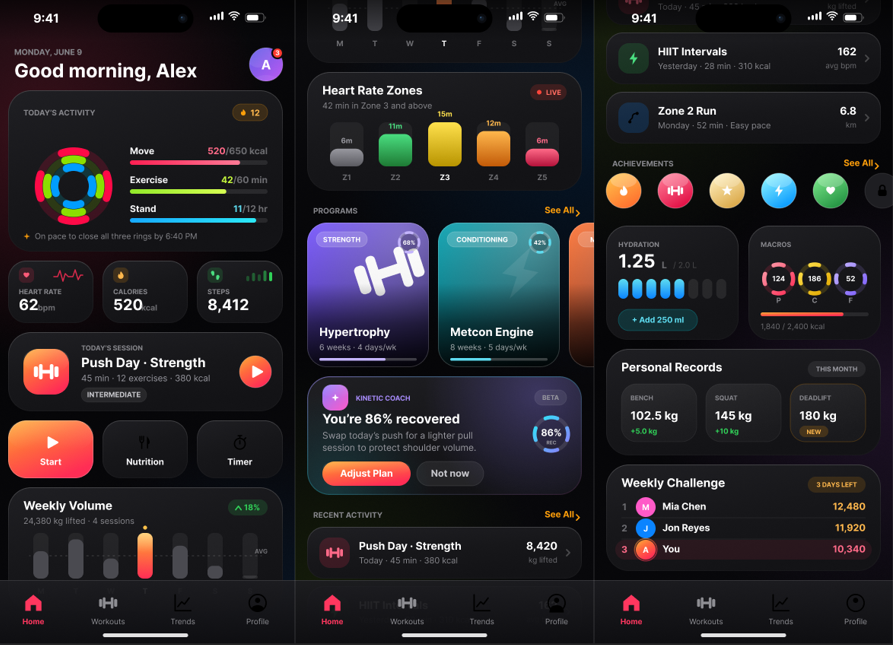
\includegraphics[width=5.5in]{screen.png}
    \caption{Alcedo Mobile Application Interface: Home Dashboard, Workout Execution, and Performance Analytics}
    \label{fig:app-screens}
\end{figure}

\subsection{System Architecture and Component Ecosystem}
The complete Alcedo platform is structured as a multi-tier client-server architecture consisting of a cross-platform mobile application, two specialized backend services, and a supplementary web portal:
\begin{enumerate}
    \item \textbf{Mobile Client Application (\textit{app/}):} Cross-platform frontend application developed using React Native 0.86, React 19, and Expo SDK 57 in TypeScript. It provides the primary user interface, local relational persistence via SQLite and Drizzle ORM, state management via Redux Toolkit, and secure token storage.
    \item \textbf{Modern Application Backend (\textit{backend-v2/}):} Modular RESTful server built on NestJS 11 and MongoDB 8 (Mongoose ODM). It handles user identity management, profile operations, workout synchronization contracts with idempotency keys, feature capability flags, and administrative site configurations.
    \item \textbf{Legacy Support Service (\textit{backend/}):} Pre-existing ASP.NET Core 10 backend supporting legacy SignalR real-time hubs and cryptographic messaging, maintained as an external dependency.
    \item \textbf{Web Portal (\textit{website/}):} Supplementary web interface built on Next.js 16 and Tailwind CSS for account management and administrative configurations.
\end{enumerate}

The high-level architectural relationship between the mobile client and supporting backend services is depicted in Figure~\ref{fig:sys-arch-flow}.

\begin{figure}[htbp]
    \centering
    \framebox[\textwidth]{
        \begin{minipage}{0.92\textwidth}
        \vspace{8pt}
        \centering
        \textbf{[Client Layer --- Mobile Device (iOS / Android)]}\\[3pt]
        \textit{Expo SDK 57 / React Native 0.86 (TypeScript 6.0)}\\
        \fbox{Expo Router Routes (24 Screens)} $\longrightarrow$ \fbox{Redux Toolkit (11 Slices)} $\longrightarrow$ \fbox{SQLite + Drizzle ORM (17 Tables)}\\
        \fbox{SecureStore (JWT Tokens)} $\longleftrightarrow$ \fbox{Authenticated Fetch Client (Single-Flight 401 Refresh)}\\[8pt]
        $\Big\Downarrow$ \textit{HTTPS / REST (Dual Base-URL Routing)} $\Big\Downarrow$\\[8pt]
        \begin{tabular}{c@{\hspace{0.4in}}c}
            \textbf{[Modern Backend Tier]} & \textbf{[Legacy Backend Tier]} \\
            \fbox{\parbox{2.3in}{\centering \textbf{backend-v2 (NestJS 11 + MongoDB)}\\
            User Management (\textit{/api/users/me})\\
            Workout Sync Contracts (\textit{/api/workouts})\\
            Feature Flags (\textit{/api/features})\\
            Admin Config (AES-256-GCM)}} &
            \fbox{\parbox{2.3in}{\centering \textbf{backend (.NET Core 10 + Postgres)}\\
            SignalR AI Chat Hubs\\
            Legacy Social Messaging\\
            Pre-existing Upstream Baseline}}
        \end{tabular}
        \vspace{8pt}
        \end{minipage}
    }
    \caption{Architectural Block Diagram and Data Flow of Project Alcedo}
    \label{fig:sys-arch-flow}
\end{figure}

\subsection{Technology Stack Summary}
The technological stack utilized across the design, implementation, and verification of Project Alcedo is detailed in Table~\ref{tab:tech-stack}.

\begin{table}[htbp]
    \centering
    \caption{Technology Stack of Project Alcedo}
    \label{tab:tech-stack}
    \begin{tabular}{|l|l|p{3.3in}|}
        \hline
        \textbf{Layer / Domain} & \textbf{Technology} & \textbf{Role and Architectural Function} \\
        \hline
        Mobile Framework & React Native 0.86 & Native cross-platform rendering engine \\
        Application Runtime & Expo SDK 57 & Unified build tooling, APIs, and Hermes engine \\
        Language & TypeScript 6.0 & Compile-time type safety across client and server \\
        Navigation Engine & Expo Router 57 & Declarative, file-based routing and deep-linking \\
        State Management & Redux Toolkit & Predictable single source of truth with middleware \\
        Local Embedded DB & SQLite & Embedded ACID-compliant client database engine \\
        Client-Side ORM & Drizzle ORM & Type-safe relational schema modeling and migrations \\
        Secure Storage & Expo SecureStore & Hardware-backed Keychain/KeyStore cryptographic vault \\
        Backend Framework & NestJS 11 & Modular, enterprise-grade TypeScript server \\
        Database Engine & MongoDB 8 & Scalable document-oriented NoSQL database \\
        Server-Side ODM & Mongoose 8 & Schema validation, indexing, and data models \\
        Testing Tooling & Vitest / Jest & Unit testing, component simulation, and API specs \\
        Static Code Analysis & Oxlint / ESLint & Code style enforcement, formatting, and linting \\
        \hline
    \end{tabular}
\end{table}

% ---------------------------------------------------------------------
\section{Tasks/Activities Performed}
This section provides an in-depth technical discussion of the software engineering activities executed during the internship, organized by architectural domain.

\subsection{Development Environment and Tooling Configuration}
The initial phase required configuring a standardized, reproducible mobile development environment. The client application configuration is defined in \textit{app/package.json} under the private package name \textit{alcedo-react}. 

Key development tooling configurations included:
\begin{itemize}
    \item \textbf{TypeScript Configuration:} Enforcing strict compiler checks via \textit{tsconfig.json} with \textit{strict: true}, \textit{strictNullChecks: true}, and \textit{noUncheckedIndexedAccess: true}. Path mapping aliases were established to decouple module resolution (e.g., \textit{@/*} mapping to \textit{src/*}).
    \item \textbf{Metro and Babel Bundler Setup:} Configured Metro bundler with SVG transformer plugins and path shims supporting styled-components on the Hermes JavaScript engine.
    \item \textbf{Static Analysis Tooling:} Integrated Oxlint and ESLint pipelines paired with Oxfmt formatters to enforce code hygiene and eliminate formatting variances across development commits.
\end{itemize}

\subsection{Reusable Interface Components and Design System}
To ensure interface consistency across 24 screens, a comprehensive foundation component library comprising 82 modular component files was constructed under \textit{app/src/components/presentation/foundation/}. 

The design system is anchored by the centralized design token specification in \textit{app/src/styles/theme.ts} (spanning 947 lines of code and 192 named typography definitions). The design tokens formalize:
\begin{itemize}
    \item \textbf{Color Palettes:} Semantic definitions for primary brand accents, container surfaces, borders, error states, and high-contrast text across Light, Dark, and true-black OLED display modes.
    \item \textbf{Typography Scale:} Responsive typographic hierarchies with explicit font sizes, line heights, and weights for display headers, section titles, card labels, and data tabular numbers.
    \item \textbf{Component Library:} Standardized atomic controls including \textit{AppButton} (primary, tonal, outlined, text variants), \textit{Card} containers, form input text fields with validation states, sheet selection dialogs, modal pickers, chip filters, and custom SVG bottom tab bar icons.
\end{itemize}

\subsection{Navigation and Screen Implementation}
Application navigation was implemented using Expo Router under \textit{app/src/app/}, organizing 49 individual route files into a cohesive hierarchy. The application root is wrapped by a root stack navigator in \textit{\_layout.tsx}, orchestrating top-level modal screens (such as exercise search, workout editor, and diff-save) over the core tab navigator.

The bottom tab navigator organizes five distinct operational tabs:
\begin{enumerate}
    \item \textbf{Workout Tab (\textit{(session)}):} Hub for initiating planned workout sessions, logging live active workouts, inspecting set history, and reviewing post-workout accomplishment summaries.
    \item \textbf{Feed Tab (\textit{feed}):} Displays social timeline posts, shared workout accomplishments, user profiles, and post details.
    \item \textbf{Stats Tab (\textit{stats}):} Analytical dashboards presenting longitudinal volume heatmaps, personal record progression, and exercise-specific strength curves.
    \item \textbf{History Tab (\textit{history}):} Interactive monthly training calendars, historical session review cards, and historical workout log editors.
    \item \textbf{Settings Tab (\textit{settings}):} Comprehensive configuration hub encompassing user profile management, display theme selectors, measurement unit toggles, local backup export/import tools, and backend connection diagnostic editors.
\end{enumerate}

A comprehensive inventory of the twenty-four primary tracked application screens is presented in Table~\ref{tab:screen-inventory}.

\begin{table}[htbp]
    \centering
    \caption{Primary Application Screen Inventory and Route Mapping}
    \label{tab:screen-inventory}
    \begin{tabular}{|c|l|l|p{2.6in}|}
        \hline
        \textbf{No.} & \textbf{Screen Identifier} & \textbf{Tab / Route Path} & \textbf{Functional Purpose} \\
        \hline
        1 & Home Dashboard & \textit{(session)/index} & Workout streaks, quick start, active plans \\
        2 & Active Workout & \textit{(session)/session/index} & Live set logging, rest timer, exercise swap \\
        3 & Post-Workout Summary & \textit{(session)/session/post} & Volume totals, PR badges, session notes \\
        4 & Workout Editor & \textit{workout-editor} & Blueprint builder, target reps/sets editor \\
        5 & Exercise Editor & \textit{exercise-editor} & Custom exercise name, muscle groups, equipment \\
        6 & Plan Diff-Save & \textit{diff-save} & Visual plan diffing and update reconciliation \\
        7 & Exercise Search & \textit{exercise-search} & Filtered catalog search by equipment and muscle \\
        8 & Exercise History & \textit{exercise-history} & Historical 1RM trends and set log history \\
        9 & Manage Exercises & \textit{settings/manage-exercises} & Custom exercise library administration \\
        10 & Feed Timeline & \textit{feed/index} & Community timeline and post feed \\
        11 & Feed Post Detail & \textit{feed/item/[id]} & Post inspection, reactions, and comments \\
        12 & Feed Share Composer & \textit{feed/share} & Share workout accomplishments to feed \\
        13 & Profile Editor & \textit{feed/profile-editor} & User display name, bio, and avatar settings \\
        14 & Shared Item Detail & \textit{feed/shared-item/[id]} & Deep-linked shared workout inspection \\
        15 & History Calendar & \textit{history/index} & Monthly workout calendar and week list \\
        16 & History Session Edit & \textit{history/edit} & Retroactive editing of completed workouts \\
        17 & Trends Dashboard & \textit{stats/index} & Volume heatmaps and weekly frequency graphs \\
        18 & Exercise Stats List & \textit{stats/exercise-list} & Per-exercise performance metric list \\
        19 & Expanded Stats & \textit{stats/expanded-weighted} & Detailed graphical progression curves \\
        20 & Settings Home & \textit{settings/index} & Primary user configuration hub \\
        21 & Preferences & \textit{settings/preferences} & Units (kg/lb), sound, and rest timer options \\
        22 & Notifications & \textit{settings/notifications} & Workout reminders and system alert toggles \\
        23 & Backup and Restore & \textit{settings/backup-and-restore} & Local JSON export/import and cloud sync \\
        24 & Backend Diagnostics & \textit{settings/backends/index} & Multi-server routing and capability probe \\
        \hline
    \end{tabular}
\end{table}

\subsection{State Management with Redux Toolkit}
Client-side operational state was architected using Redux Toolkit (RTK) across 11 domain slices located in \textit{app/src/store/slices/}. The store maintains independent state slices for:
\begin{itemize}
    \item \textit{Session Slice:} Active workout state, current exercise index, completed sets, active rest timer countdown, and session pause states.
    \item \textit{History Slice:} Cached completed workout summaries, calendar dates, and query filters.
    \item \textit{Exercises Slice:} Cached exercise definitions, user-created custom movements, and search indices.
    \item \textit{Preferences Slice:} User interface configurations, active color theme (dark/light/OLED), measurement units, and timer preferences.
    \item \textit{Backends Slice:} Registered server endpoints, active URL assignments, and probed feature availability flags.
    \item \textit{Auth Slice:} Active session state, authenticated user metadata, and token validity flags.
\end{itemize}

To coordinate complex asynchronous workflows without cluttering UI components, a custom listener middleware (\textit{addEffect}) was configured. The middleware intercepts specific action dispatches (e.g., completing a set or updating preferences) and triggers non-blocking secondary effects, including atomic SQLite persistence and cache invalidation.

\subsection{Local Data Storage, SQLite, and Drizzle ORM}
To deliver a true offline-first user experience, local persistence was implemented using an embedded SQLite database managed via Drizzle ORM under \textit{app/src/db/}. The database schema comprises 17 relational tables, organized with strict foreign key constraints and indexed queries.

The database tables encompass:
\begin{itemize}
    \item Core workout tables: \textit{sessions}, \textit{recorded\_exercises}, \textit{recorded\_sets}, \textit{cardio\_records}.
    \item Blueprint planning tables: \textit{program\_blueprints}, \textit{session\_blueprints}, \textit{exercise\_blueprints}, \textit{set\_blueprints}.
    \item Exercise definitions: \textit{exercise\_descriptors}, \textit{muscle\_groups}, \textit{equipment\_categories}.
    \item Synchronization and metadata: \textit{sync\_journal}, \textit{tombstones}, \textit{schema\_migrations}.
\end{itemize}

Schema evolution is governed by nine sequential SQL migrations. When the application initializes, a database bootstrapper verifies the active user-version pragma, executes pending migrations within a transactional block, and verifies schema integrity. For hardware-backed secret management, sensitive JWT tokens are stored outside SQLite using \textit{Expo SecureStore}, ensuring cryptographic isolation.

\subsection{Frontend--Backend Integration and Security Lifecycle}
Client--server communication was engineered to satisfy strict security and reliability standards. Network requests to the modern backend are mediated by a centralized client wrapper (\textit{authenticated-fetch.ts}). 

The integration architecture implements key security mechanisms:
\begin{itemize}
    \item \textbf{Stateless Token Injection:} Outgoing HTTP requests automatically inject the stored JWT access token into the standard \textit{Authorization: Bearer <token>} header.
    \item \textbf{Single-Flight 401 Refresh Interceptor:} When an access token expires, backend endpoints respond with HTTP 401 Unauthorized. The \textit{authenticated-fetch} wrapper intercepts this response, pauses concurrent outgoing network requests via an internal promise-based mutex, executes a single refresh request to \textit{/api/auth/refresh} using the securely stored refresh token, updates the token cache, and replays the queued requests. This pattern prevents duplicate, racing refresh requests when multiple UI queries fail concurrently.
    \item \textbf{Backend Capability Discovery:} The mobile client queries \textit{GET /api/features} through \textit{backend-probe.ts} to evaluate dynamic server capabilities (such as feed availability, backup support, and AI planning), gracefully adapting the client interface based on active server flags.
\end{itemize}

\subsection{User Management Module}
The User Management module in \textit{backend-v2/src/users/} provides profile management services for authenticated gym members. Developed with NestJS and MongoDB, the module implements:
\begin{itemize}
    \item Profile data retrieval via \textit{GET /api/users/me}, returning the member's profile attributes, account creation timestamp, and subscription entitlement status.
    \item Profile updates via \textit{PATCH /api/users/me}, allowing members to update display names, bio descriptions, and user preferences.
    \item Strict request validation enforced via class-validator DTOs (\textit{UpdateUserDto}), sanitizing inputs and rejecting malformed payloads before database execution.
\end{itemize}

\subsection{Workout Management and Synchronization Contracts}
The Workout Management service in \textit{backend-v2/src/workouts/} implements the server-side business logic for storing, validating, and synchronizing gym workout sessions.

Key technical components include:
\begin{itemize}
    \item \textbf{Workout CRUD Endpoints:} Endpoints for creating, fetching, modifying, and soft-deleting workout session documents.
    \item \textbf{Compare-and-Set Versioning:} Each workout document incorporates a monotonic version integer. Updates must present the matching expected version, preventing accidental overwrite of concurrent edits.
    \item \textbf{Soft Deletes and Tombstones:} Deleted sessions generate server-side tombstone records containing deletion timestamps, ensuring downstream synchronization cycles can reliably propagate deletions to client databases.
    \item \textbf{Batch Synchronization Contracts:} The backend exposes batch push and pull endpoints (\textit{/api/workouts/sync}) featuring idempotency key tracking. While the mobile client's production runtime currently executes local workout storage with client-side preparation, the backend sync contracts were validated and prepared for future enterprise multi-device replication.
\end{itemize}

\subsection{Feature Management and Runtime Configuration}
Feature Management is implemented through a two-tiered system operating across backend-v2 and the mobile client:
\begin{enumerate}
    \item \textbf{Public Feature Capability Flags:} The endpoint \textit{GET /api/features} distributes a public feature map reporting boolean availability flags (e.g., \textit{feed}, \textit{aiPlanner}, \textit{backup}, \textit{sharing}). The mobile app's \textit{backend-probe.ts} consumes this endpoint to adapt the UI dynamically.
    \item \textbf{Encrypted Site Configuration:} An administrative configuration service in \textit{backend-v2/src/site-config/} manages an allowlist of 16 system configuration keys. Sensitive secrets (such as external API keys) are encrypted at rest using AES-256-GCM authenticated encryption and masked during administrative read operations.
\end{enumerate}

\subsection{Testing, Quality Assurance, and Debugging}
Quality assurance was conducted systematically throughout development, combining automated unit tests, component simulations, static analysis, and emulator verification. The test suite distribution across system layers is summarized in Table~\ref{tab:test-distribution}.

\begin{table}[htbp]
    \centering
    \caption{Automated Quality Assurance and Test Suites by System Layer}
    \label{tab:test-distribution}
    \begin{tabular}{|l|l|c|p{2.8in}|}
        \hline
        \textbf{Layer} & \textbf{Framework} & \textbf{Suites / Specs} & \textbf{Verification Scope} \\
        \hline
        Mobile Client (\textit{app}) & Vitest & 140 Spec Files & Component simulations (51), Redux store (34), data models (25), services (19), utils (7), database (4) \\
        \hline
        Mobile Property Tests & Fast-Check & Embedded & Generative property tests for workout calculation and math \\
        \hline
        Mobile E2E Workflows & Maestro & 6 Flow Specs & Critical user journeys: onboard, log workout, view history \\
        \hline
        Backend Service & Jest & 19 Test Suites & 194 test blocks covering users, workouts, auth, and features \\
        \hline
        Static Type Checking & TypeScript & Whole Project & Strict mode compilation checking zero type errors \\
        \hline
        Code Linter / Formatter & Oxlint / ESLint & Whole Project & Code style, hook dependencies, and formatting checks \\
        \hline
    \end{tabular}
\end{table}

Quality gates were executed manually prior to commit integration, verifying typecheck cleanliness, lint passing, and test suite execution. Commit messages systematically recorded running test totals (progressing from 1,472 to over 2,140 passing tests) and documented verification boundaries.

\subsection{Version Control and Branch Management Workflow}
Software development followed disciplined Git version control workflows. Work was structured using feature branches, conventional commit semantics, and structured commit bodies detailing specific file modifications, executed test commands, and verification outputs. 

During major branch integrations, formal merge programmes were executed using documented merge ledgers (\textit{merge\_ledger.md}) and hazard registers. Pre-merge snapshots and safety tags were created to mitigate regression risks, ensuring clean branch consolidation across multi-thousand-line updates without architectural degradation.
% =====================================================================
%  Chapter 4 — Conclusion and Learning Outcomes
%  Structure fixed by docs/guidelines/guidelines.md (section 3, item 4):
%    4.1 Conclusion
%    4.2 Learning Outcome
%  The guideline adds: "Students should be able to relate and contextualize
%  the above-mentioned concepts with their project work/activities done
%  during internship at the host organization."
%
%  Content sources: docs/project_detail/11_report_mapping.md (Chapter 4 row)
%                    data/information/role_and_responsibility.md (final para)
% =====================================================================
\chapter{Conclusion and Learning Outcomes}

% ---------------------------------------------------------------------
\section{Conclusion}
% TODO Summarise the internship against its objectives: what the application
% now does, what was delivered, and what the experience showed about working
% in a real project with a mentor and a client.
% Anchor it in the feature inventory (project_detail/01_project_overview.md
% section 4) rather than in adjectives.

% ---------------------------------------------------------------------
\section{Learning Outcome}
% TODO Technical and professional learning, tied to work actually done:
%   - component-based UI implementation and design systems
%   - state management and offline-first persistence
%   - API integration and authentication flows
%   - backend module development (users, workouts, feature configuration)
%   - automated testing at three levels and disciplined debugging
%   - version control, branching and a documented merge
% Then the personal outcomes: working to a deadline, taking feedback,
% communicating with non-technical staff (trainers, front desk, management).
% The final paragraph of data/information/role_and_responsibility.md may be
% adapted as the closing paragraph.
%
% Every claim here must be traceable to project_detail/; do not add skills
% that are not evidenced in the project.

% ---------------------------------------------------------------------
%  Back matter — continues the arabic numbering
% ---------------------------------------------------------------------
% =====================================================================
%  References (APA 7th edition)
%
%  NOTE: \begin{thebibliography} issues its own chapter heading, taken from
%  \bibname. The heading is therefore renamed below instead of adding a
%  manual \chapter*{References} — two headings would otherwise collide.
%
%  HOW TO ADD A SOURCE — follow this exactly, or the in-text citation will
%  not match APA (see docs/imp/plan.md section 6):
%
%    \bibitem[Surname (Year)]{key}
%    Surname, A. A. (Year). \textit{Title of the work}. Publisher.
%
%  For three or more authors the label must use "et al.":
%    \bibitem[Abras et al. (2004)]{key}
%
%  Then cite in the text with \citep{key} -> (Surname, Year)
%                              or  \citet{key} -> Surname (Year)
%
%  Every entry here must be a real, checkable source that is actually cited
%  in the text. If a source was read but not cited, it belongs in
%  bibliography.tex instead.
% =====================================================================
\clearpage
\renewcommand{\bibname}{References}
\addcontentsline{toc}{chapter}{References}

\begin{thebibliography}{99}

% ---------------------------------------------------------------------
% TODO: replace this scaffold entry with the real literature used in
% section 2.5. Delete it before submission if it is not cited.
%
% These two are placeholders showing the required format only — verify each
% against the publisher before keeping it.
% ---------------------------------------------------------------------

\bibitem[NACE (2022)]{nace2022}
National Association of Colleges and Employers. (2022). \textit{Position statement: U.S. internships and compensation}. National Association of Colleges and Employers.

\bibitem[Parveen (2012)]{parveen2012}
Parveen, H. (2012). A study of internship program and its impact on student career choices. \textit{Journal of Education and Practice}, \textit{3}(15), 182--189.

\bibitem[Tribhuvan University (2022)]{tu2022curriculum}
Tribhuvan University. (2022). \textit{Bachelor of Science in Computer Science and Information Technology (B.Sc. CSIT) curriculum}. Institute of Science and Technology, Tribhuvan University.

\bibitem[Frain (2022)]{frain2022}
Frain, B. (2022). \textit{Responsive web design with HTML5 and CSS} (4th ed.). New Riders.

\bibitem[Abras et al. (2004)]{abras2004}
Abras, P., Maloney-Krichmar, D., \& Preece, J. (2004). User-centered design. In W. Bainbridge (Ed.),
\textit{Encyclopedia of human-computer interaction} (pp. 445--456). Sage Publications.

\bibitem[Banks \& Porcello (2020)]{banks2020learning}
Banks, A., \& Porcello, E. (2020). \textit{Learning React: Modern patterns for developing React apps} (2nd ed.). O'Reilly Media.

\bibitem[Biorn-Hansen et al. (2020)]{biorn2020survey}
Bi\o rn-Hansen, A., Gr\o nli, T.-M., \& Ghinea, G. (2020). A survey and taxonomy of core concepts and challenges in cross-platform mobile development. \textit{ACM Computing Surveys}, \textit{53}(4), 1--34. https://doi.org/10.1145/3396860

\bibitem[Fielding (2000)]{fielding2000}
Fielding, R. T. (2000). \textit{Architectural styles and the design of network-based software architectures} (Doctoral dissertation). University of California, Irvine.

\bibitem[Jones et al. (2015)]{jones2015jwt}
Jones, M., Bradley, J., \& Sakimura, N. (2015). \textit{JSON Web Token (JWT)} (RFC 7519). Internet Engineering Task Force. https://doi.org/10.17487/RFC7519

\bibitem[Kleppmann (2017)]{kleppmann2017}
Kleppmann, M. (2017). \textit{Designing data-intensive applications: The big ideas behind reliable, scalable, and maintainable systems}. O'Reilly Media.

\bibitem[Martin (2008)]{martin2008clean}
Martin, R. C. (2008). \textit{Clean code: A handbook of agile software craftsmanship}. Prentice Hall.

\bibitem[Nielsen (1994)]{nielsen1994}
Nielsen, J. (1994). \textit{Usability engineering}. Morgan Kaufmann.

\bibitem[Tilkov \& Vinoski (2010)]{tilkov2010node}
Tilkov, S., \& Vinoski, S. (2010). Node.js: Using JavaScript to build high-performance network programs. \textit{IEEE Internet Computing}, \textit{14}(6), 80--83. https://doi.org/10.1109/MIC.2010.145

% ---------------------------------------------------------------------
% Likely additions — confirm each is real and actually cited:
%   Expo documentation            https://docs.expo.dev
%   React Native documentation    https://reactnative.dev/docs/getting-started
%   expo-router documentation     https://docs.expo.dev/router/introduction/
%   Redux Toolkit documentation  https://redux-toolkit.js.org/introduction/getting-started
%   Drizzle ORM documentation    https://orm.drizzle.team/docs/overview
%   SQLite documentation          https://www.sqlite.org/docs.html
%   NestJS documentation          https://docs.nestjs.com/
%   MongoDB / Mongoose docs       https://mongoosejs.com/docs/
%   JWT (RFC 7519)                https://datatracker.ietf.org/doc/html/rfc7519
%   Material Design 3             https://m3.material.io/
%   Nielsen, J. (1994). Usability engineering. Morgan Kaufmann.
%   Fielding, R. (2000). Architectural styles and the design of network-based
%     software architectures (Doctoral dissertation, University of California,
%     Irvine). https://ics.uci.edu/~fielding/pubs/dissertation/top.htm
%   W3C WCAG 2.2 https://www.w3.org/TR/WCAG22/
% ---------------------------------------------------------------------

\end{thebibliography}

% Formatting note: hanging indent is inherited from the report class. If the
% reference list needs a 0.5in hanging indent (APA), add before
% \begin{thebibliography}:
%   \setlength{\itemsep}{0pt}
% and check the result visually.
% =====================================================================
%  Bibliography
%  Optional section (guidelines item 9): works that were read during the
%  internship but are NOT cited in the report.
%
%  If nothing ends up here, delete BOTH this file and its \input line in
%  main.tex — an empty "Bibliography" page looks worse than none.
% =====================================================================
\clearpage
\chapter*{Bibliography}
\addcontentsline{toc}{chapter}{Bibliography}

\vspace{0.3in}

% TODO: list uncited but consulted sources, same APA format as
% back-matter/references.tex. Because these entries are not cited, do not
% use \bibitem labels that \citep would resolve; a simple hanging-indent list
% is enough, for example:
%
%   \begin{list}{}{\setlength{\leftmargin}{0.5in}\setlength{\itemindent}{-0.5in}}
%     \item Surname, A. A. (Year). \textit{Title}. Publisher.
%   \end{list}
%
% Candidate sources that were part of this project but may not be cited in
% the text: the repository's own README, AGENTS.md, the design ledgers and
% the merge ledger. Note that internal project documents are usually NOT
% listed as bibliography entries; they are cited as project artefacts in
% the text instead. Decide deliberately.
% =====================================================================
%  Appendices (guidelines item 10: screenshots)
%
%  In accordance with company confidentiality policy, internal project
%  details (repository structure, database schemas, and source code
%  extracts) are omitted. Only user-facing interface screens are included
%  (Appendix A).
% =====================================================================
\clearpage
\appendix
\addcontentsline{toc}{chapter}{APPENDIX}
\addtocontents{toc}{\protect\setcounter{tocdepth}{-1}}

% =====================================================================
%  Appendix A — Application User Interface Screens
% =====================================================================
\chapter{Application User Interface Screens}
\label{app:screenshots}

This appendix presents the primary user interface screens of the Alcedo mobile application. Figure~\ref{fig:app_screens_appendix} displays the core screens.

\begin{figure}[htbp]
    \centering
    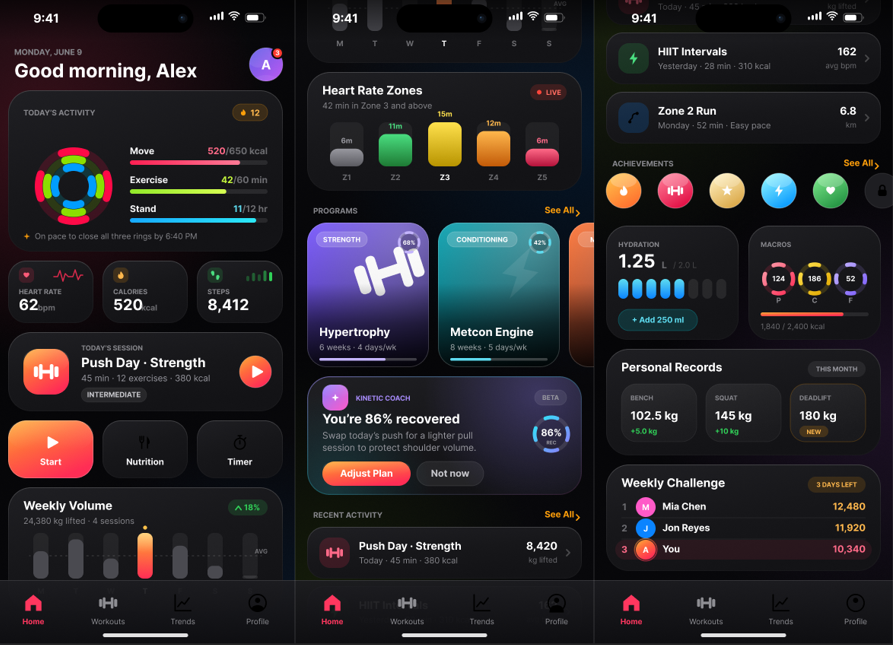
\includegraphics[width=5.5in]{screen.png}
    \caption{Alcedo Core Screens: Home Dashboard, Workout Execution, and Performance Analytics}
    \label{fig:app_screens_appendix}
\end{figure}

\section{Screen Overview}
The application encompasses twenty-four screens organized across five navigation tabs:

\subsection{Workout and Session Tracking}
\begin{itemize}
    \item \textbf{Home Dashboard:} Displays workout streaks, quick-start launcher, and assigned routine blueprints.
    \item \textbf{Live Workout Execution:} Set-by-set recording with weight/rep inputs, set-type toggles, rest timer, and exercise replacement.
    \item \textbf{Post-Workout Summary:} Session metrics including total tonnage, sets, reps, duration, and PR badges.
    \item \textbf{Workout Blueprint Editor:} Interface for constructing multi-week training programs.
    \item \textbf{Plan Diff-Save:} Side-by-side visual comparison when modifying existing routines.
\end{itemize}

\subsection{Exercise Library}
\begin{itemize}
    \item \textbf{Exercise Search:} Catalog search filtered by muscle group and equipment type.
    \item \textbf{Exercise Detail and History:} Execution guidance and historical weight/rep logs.
    \item \textbf{Custom Exercise Creator:} Registration of custom exercises with muscle and equipment classifications.
\end{itemize}

\subsection{History and Calendar}
\begin{itemize}
    \item \textbf{Training Calendar:} Monthly calendar with activity indicators and weekly workout list.
    \item \textbf{Session Editor:} Retroactive editing of completed workout logs.
\end{itemize}

\subsection{Performance Analytics}
\begin{itemize}
    \item \textbf{Trends Dashboard:} Training volume heatmaps and frequency graphs.
    \item \textbf{Progression Curves:} Estimated 1RM charts and muscle group load distribution.
\end{itemize}

\subsection{Settings and Configuration}
\begin{itemize}
    \item \textbf{Settings Hub:} User profile, display preferences, and diagnostics.
    \item \textbf{Theme Selection:} Light, Dark, and OLED mode switching with sound and unit toggles.
    \item \textbf{Backup and Restore:} Local JSON export/import and data sharing.
    \item \textbf{Backend Diagnostics:} Server URLs, token states, and feature probe results.
\end{itemize}


\end{document}
